\documentclass[12pt]{article}

\title{Hodge star operator in Euclidean dimension $n \ge 3$ as applied to the matrix determinant}
\author{S. Halayka\footnote{sjhalayka@gmail.com}}
\date{\today\;\currenttime}

\usepackage{datetime}
\usepackage{listings}
\usepackage{cite}
\usepackage{xcolor}
\usepackage{graphicx}
\usepackage{setspace}
\usepackage{amsmath}
\usepackage{url}
\usepackage[margin=0.8in]{geometry}
\usepackage{listings}
\usepackage{xcolor}



\lstset { %
    language=C++,
    backgroundcolor=\color{black!5}, % set backgroundcolor
    basicstyle=\ttfamily\footnotesize,% basic font setting
    showstringspaces=false,
}


%\doublespace

%\usepackage[]{lineno}
%\linenumbers


\begin{document}



 
\maketitle

\begin{abstract}
This paper contains a short introduction to the Hodge star operator in dimension $n \ge 3$.
The main focus is on some C++ code.
\end{abstract}




\section{Application: the matrix determinant}

In this paper, we focus on the Hodge star operator in dimension $n \ge 3$.
The beginnings of this paper/code were supplied by the Claude AI.
Various changes to the code were needed in order for it to operate properly, but the kernel of the idea remains the same.
The chat log is at:

\url{https://claude.ai/chat/3caf4077-28b5-497f-b704-1b0c336a104d}

The main goal is to acquaint the coder with the basic idea behind the Hodge star operator in $n$-D. 
The operator accepts $(n - 1)$ $n$-vectors as input, and outputs one $n$-vector.
For instance, where $n = 3$, the $3$-D Hodge star operator accepts $(n - 1) = $ two $3$-vectors as input.
Using C++ templates, the abstraction to any $n \ge 3$ is provided.
This Hodge star operator is used to calculate the matrix determinant.







\section{Code}

Here we include the Eigen linear algebra library, as well as various parts of the standard library:
\begin{lstlisting}
#include <Eigen/Dense>
using namespace Eigen;

#include <iostream>
#include <vector>
#include <numeric>
#include <string>
#include <sstream>
#include <algorithm>
#include <array>
using namespace std;
\end{lstlisting}

Here we define the vector class, where the data type is T (e.g., double), and N is the dimension:
\begin{lstlisting}
template<class T, size_t N>
class Vector_nD
{
public:
  array<T, N> components;

  // Levi-Civita symbol -- get the sign of permutation
  static signed char permutation_sign(const array<int, (N - 1)>& perm)
  {
    bool sign = true;

    for (int i = 0; i < (N - 2); i++)
      for (int j = i + 1; j < (N - 1); j++)
        if (perm[i] > perm[j])
          sign = !sign;

    if (sign)
      return 1;
    else
      return -1;
  }

  Vector_nD(const array<T, N>& comps) : components(comps)
  {
  }

  Vector_nD(void)
  {
    components.fill(0.0);
  }

  T operator[](size_t index) const
  {
    return components[index];
  }

\end{lstlisting}

Here we make a static Hodge star operator function that takes in $(n - 1)$ $n$-vectors.
This function returns one $n$-vector:
\begin{lstlisting}

  // Hodge star operator
  static Vector_nD star(const vector<Vector_nD<T, N>>& vectors)
  {
    if (vectors.size() != (N - 1))
    {
      cout << "nD operation requires (n - 1) input vectors" << endl;
      return Vector_nD<T, N>();
    }

    array<T, N> result;

    for (size_t i = 0; i < N; i++)
      result[i] = 0.0;

    // These are the indices we'll use for each component calculation
    array<int, (N - 1)> base_indices;

    for (int i = 0; i < (N - 1); i++)
      base_indices[i] = i;

    // Skip k in our calculations - 
    // this is equivalent to removing the k-th column
    // For each permutation of the remaining (N - 1) indices
    for (int k = 0; k < N; k++)
    {
      do
      {
        // Calculate sign of this term
        const signed char sign = permutation_sign(base_indices);

        // Calculate the product for this permutation
        T product = 1.0;
        ostringstream product_oss;

        for (int i = 0; i < (N - 1); i++)
        {
          const int col = base_indices[i];

          // Adjust column index if it's past k
          int actual_col = 0;

          if (col < k)
            actual_col = col;
          else
            actual_col = col + 1;

          product_oss << "v_{" << i << actual_col << "} ";

          product *= vectors[i][actual_col];
        }

        if (sign == 1)
          cout << "x_{" << k << "} += " << product_oss.str() << endl;
        else
          cout << "x_{" << k << "} -= " << product_oss.str() << endl;

        result[k] += sign * product;

      } while(next_permutation(
          base_indices.begin(), 
          base_indices.end()));
    }

    // Flip handedness
    for (size_t k = 0; k < N; k++)
      if (k % 2 == 1)
        result[k] = -result[k];

    cout << endl;

    for (int k = 0; k < N; k++)
      cout << "result[" << k << "] = " << result[k] << endl;

    cout << endl;

    if (N == 3)
    {
      // Demonstrate the traditional cross product
      double x = vectors[0][0];
      double y = vectors[0][1];
      double z = vectors[0][2];

      double rhs_x = vectors[1][0];
      double rhs_y = vectors[1][1];
      double rhs_z = vectors[1][2];

      double cross_x = y * rhs_z - rhs_y * z;
      double cross_y = z * rhs_x - rhs_z * x;
      double cross_z = x * rhs_y - rhs_x * y;

      cout << cross_x << " " << cross_y << " " << cross_z << endl << endl;
    }

    return Vector_nD(result);
  }

\end{lstlisting}

Here we have the static dot product function:
\begin{lstlisting}

  static T dot_product(const Vector_nD<T, N>& a, const Vector_nD<T, N>& b)
  {
    return inner_product(
      a.components.begin(), 
      a.components.end(), 
      b.components.begin(), 0.0);
  }
};

\end{lstlisting}

Finally, we calculate the determinant of a square matrix using the Hodge star operator and the dot product operator as defined above:
\begin{lstlisting}

template <class T, typename size_t N>
T determinant_nxn(const MatrixX<T>& m)
{
  if (m.cols() != m.rows())
  {
    cout << "Matrix must be square" << endl;
    return 0;
  }

  // We will use this N-vector later, in the dot product operation
  Vector_nD<T, N> a_vector;

  for (size_t i = 0; i < N; i++)
    a_vector.components[i] = m(0, i);

  // We will use these (N - 1) N-vectors later, 
  // in the Hodge star operation
  vector<Vector_nD<T, N>> input_vectors;

  for (size_t i = 1; i < N; i++)
  {
    Vector_nD<T, N> b_vector;

    for (size_t j = 0; j < N; j++)
      b_vector.components[j] = m(i, j);

    input_vectors.push_back(b_vector);
  }

  // Compute the Hodge star operator using (N - 1) N-vectors
  Vector_nD<T, N> result = Vector_nD<T, N>::star(input_vectors);

  // Compute the dot product
  T det = Vector_nD<T, N>::dot_product(a_vector, result);

  // These numbers should match
  cout << "Determinant:       " << det << endl;
  cout << "Eigen Determinant: " << m.determinant() << endl << endl;

  return det;
}

\end{lstlisting}

This main function is for testing the above code:
\begin{lstlisting}

int main(int argc, char** argv)
{
  srand(static_cast<unsigned int>(time(0)));

  const size_t N = 4; // Anything larger than 12 takes eons to solve for

  MatrixX<double> m(N, N);

  for (size_t i = 0; i < N; i++)
  {
    for (size_t j = 0; j < N; j++)
    {
      m(i, j) = rand() / static_cast<double>(RAND_MAX);

      if (rand() % 2 == 0)
        m(i, j) = -m(i, j);
    }
  }

  determinant_nxn<double, N>(m);

  return 0;
}
\end{lstlisting}
Here we have shown the geometric way to calculate the matrix determinant, by using the hypervolume of an $(n - 1)$-D parallelogram base, where $n \ge 3$. 
See Fig. 1.
\begin{figure} 
\centering
  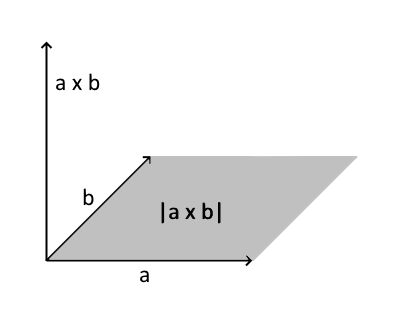
\includegraphics[width = 3 in]{parallelogram.png}
  \caption{
A $2$-D parallelogram base in $3$-D space.
Note that the Hodge star operator (e.g. $\star(a \wedge b)$) and the cross product operator (e.g. $a \times b$) are equivalent in $3$-D, after taking handedness into account.
}
\end{figure}

\section{Examples of the Hodge star operator}
For $n = 3$, where $\star(v_{0} \wedge v_{1})$:
\begin{eqnarray}
x_{0} &=& v_{01} v_{12} - v_{02} v_{11},\\
x_{1} &=& v_{00} v_{12} - v_{02} v_{10},\\
x_{2} &=& v_{00} v_{11} - v_{01} v_{10}.
\end{eqnarray}

For $n = 4$, where $\star(v_{0} \wedge v_{1} \wedge v_{2})$:
\begin{eqnarray}
x_{0} &=& 
   v_{01} v_{12} v_{23}
 + v_{02} v_{13} v_{21}
 + v_{03} v_{11} v_{22}
 - v_{01} v_{13} v_{22}
 - v_{02} v_{11} v_{23}
 - v_{03} v_{12} v_{21},\\
x_{1} &=& 
    v_{00} v_{12} v_{23}
 + v_{02} v_{13} v_{20}
  + v_{03} v_{10} v_{22}
  - v_{00} v_{13} v_{22}
 - v_{02} v_{10} v_{23}
  - v_{03} v_{12} v_{20},\\
x_{2} &=& 
v_{00} v_{11} v_{23}
  + v_{01} v_{13} v_{20}
  + v_{03} v_{10} v_{21}
- v_{00} v_{13} v_{21}
  - v_{01} v_{10} v_{23}
  - v_{03} v_{11} v_{20},\\
x_{3} &=& 
   v_{00} v_{11} v_{22}
 + v_{01} v_{12} v_{20}
 + v_{02} v_{10} v_{21}
 - v_{00} v_{12} v_{21}
 - v_{01} v_{10} v_{22}
 - v_{02} v_{11} v_{20}.
\end{eqnarray}
For $n \ge 5$, where $\star(v_{0} \wedge v_{1} \wedge v_{2} \wedge\;\cdots\;\wedge v_{(n - 2)})$, the terms become too numerous to print here.










%\begin{thebibliography}{9}





%\bibitem{nasa} Williams. NASA Mercury Fact Sheet. (2024)



%\end{thebibliography}














\end{document}









